% !TEX root = ../bachlor-arbeit.tex
Artificial Neural Networks (ANN's or short NN's) are a kind of data structure inspired by the biological neurons found in nature. They can be used to find a wide range of input output relations. One classic example is mapping pictures of hand written digits to the actual digits. Rather than explicitly programmed, NN's are trained on a dataset $(X, \, Y)$ of correct input output pairs.
\\


\begin{figure}[H]
    \centering
    \includegraphics[width=.6\linewidth]{bg_basic_nn}
    \caption{The most simple kind of NN is called densely connected or multilayer perceptron. For clarity only connections to the top most node of each layer are shown.}
    \label{fig:bg:basic_nn}
\end{figure}

\paragraph{Multilayer Perceptron}
This kind of classic NN consist of single nodes or neurons which are organized into layers. The terms node and neuron can be used interchangeably. Every node is connected to all the nodes of the previous and the next layer. For this reason the network is called dense or densely connected. Each node holds a value called activation $a$ where the activation to the first layer is the input to the network, here:
$(x_1, \, x_2, \, x_3)$.
The nodes are connected by weights $w$ which specify how much one node should influence the next and every node has a bias $b$ to control at what total input activation the node itself should become active.
To calculate the activation of a node one has to multiply all the activations of the previous layer with their respective weights $w$, add the bias $b$ and finally apply a non-linear activation function $\sigma$ as seen in Figure \ref{fig:al:act}. To describe this process mathematically we are going to use the usual index notation where superscripts specify the layer and subscripts the node. So $a^2_1$ is the activation of the first node in the second layer. To characterize a weight two subscripts are needed for the end and beginning of the connection. For the example in figure \ref{fig:bg:basic_nn} that means:

\begin{equation} \label{eq:bg:activation_example}
    a^2_1 = \sigma \qty(\sum_i w^2_{1i} \, x_i + b^2_1)
\end{equation}

\noindent
However it is more convenient to stop considering every node individually and to view the involved quantities as vectors and matrices. So that \eqref{eq:bg:activation_example} can be written as:

\begin{equation} \label{eq:bg:activation}
    \vb{a}^l = \sigma \qty(\vu{w}^l \vb{a}^{l-1} + \vb{b}^l)
\end{equation}

\begin{figure}[H]
\centering
\begin{subfigure}{.5\textwidth}
    \centering
    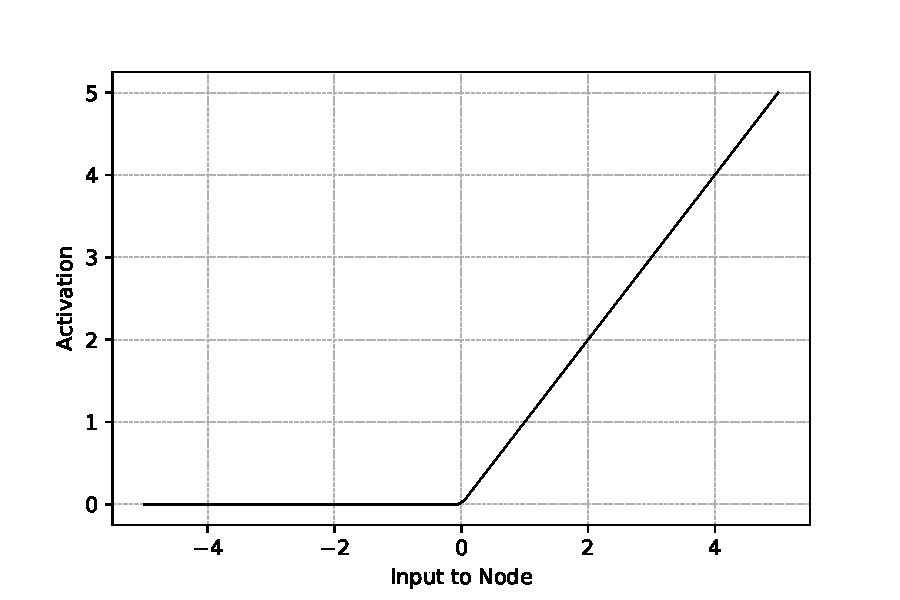
\includegraphics[width=\linewidth]{bg_relu}
    \caption{rectified linear unit (ReLu)}
    \label{}
\end{subfigure}%
\begin{subfigure}{.5\textwidth}
    \centering
    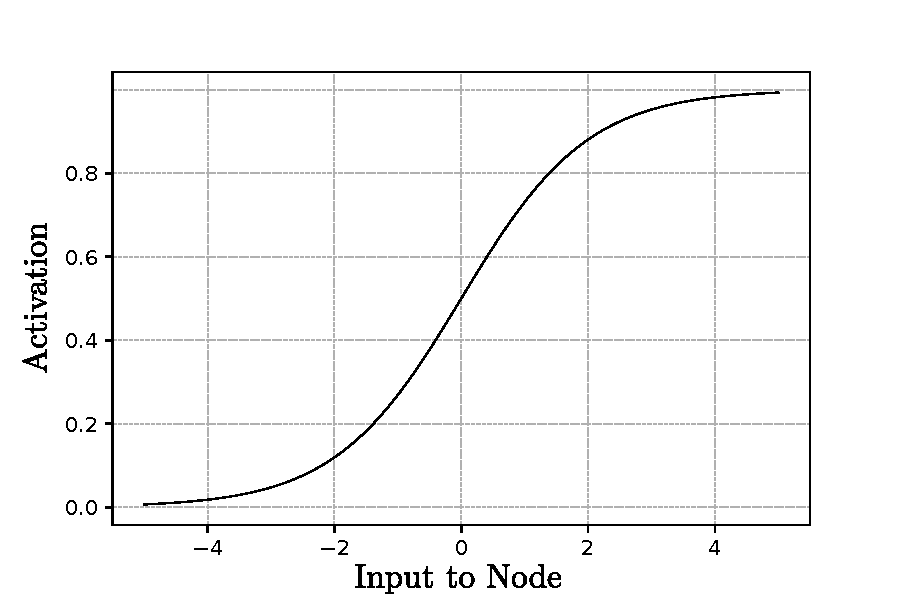
\includegraphics[width=\linewidth]{bg_sigmoid}
    \caption{sigmoid}
    \label{}
\end{subfigure}
\caption{Two examples of activation functions $\sigma$. Especially the ReLu function has a destinct on and off state similar to a biological neurons.}
\label{fig:al:act}
\end{figure}

\paragraph{Training} \label{par:training}
During training the network output $\s{NN}(\vb x) := \vb{y}' $ is calculated through repeated use of \eqref{eq:bg:activation} and is then compared with the known correct output $\vb y$ by a cost function $C = C(\vb y, \, \vb y')$. The goal of the training is to minimize this function $C$. The cost function might simply be the mean squared difference between $\vb y$ and $\vb y'$:

\begin{equation}
    C_\s{mse}(\vb y, \, \vb y') = \sum_i \qty(y_i - y_i')^2
\end{equation}

\noindent
but there are different cost functions for different kind of outputs. For example a network which predicts continuous values needs a different loss than one predicting categories. More on this in section \ref{sec:NN}. Now we can quantify how well the NN is performing but how should the weights and biases be changed to improve this performance?
Here the Algorithm \textit{Backpropagation} is used and allows an efficient approximation of the gradients for $\vb{b}^l$ and $\vu{w}^l$. These are used to gradually change the weights and biases to minimize the cost function. A comprehensive explanation of Backpropagation can be found here: \cite{backprop}.

\paragraph{Convolutional Neural Networks}
An area where NNs have been very successful is image recognition or more general computer vision but the described multilayer perceptron has a number of weaknesses for this kind of task. Let's say our input is a $n$ by $n$ gray scale image. This can be expressed as a $n \cp n$ matrix, flattened and fed into the input layer (see figure \ref{fig:bg:flatten}). But now the number of weights to the next layer $\vu{w}^2$ is $n \cdot n \cdot \qty| \boldsymbol l^2|$
which soon becomes unfeasible. As described in the section on \hyperref[sec:notation]{notation} $\boldsymbol l^2$ is here the activation vector of the second layer and not $\boldsymbol l$ squared.

\begin{figure}[H]
    \centering
    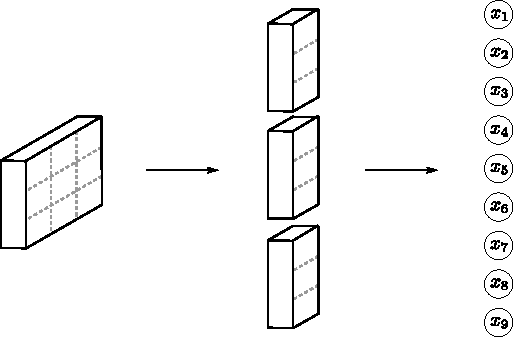
\includegraphics[width=.45\linewidth]{bg_flatten}
    \caption{Flattening of a $3\cp3$ matrix to fit the input of a multilayer perceptron.}
    \label{fig:bg:flatten}
\end{figure}

Computational limits aside there is another problem. Imagine an image with the letter T in the top right corner. If this letter moves to a different position as in figure \ref{fig:bg:convnet_T} the networks reaction will be completely different because the weights and biases involved are completely different. So the NN cannot learn the concept "letter T" independent of its position in the picture. Also the information about the distance between pixels is lost.

\begin{figure}[H]
    \centering
    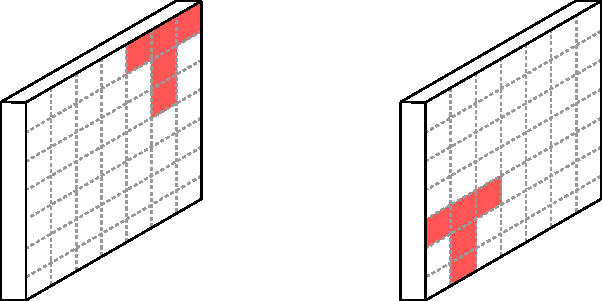
\includegraphics[width=.6\linewidth]{bg_convnet_T}
    \caption{Two pictures of a T at different positions where the red color signifies a high value in the grayscale image. After the flatten operation seen in figure \ref{fig:bg:flatten} very different nodes are active.}
    \label{fig:bg:convnet_T}
\end{figure}

These problems led to the development of a new kind of layer called \textit{Convolution}. A fixed size squared matrix called \textit{kernel} is shifted over the matrix and at every position the the point wise product between kernel and matrix is calculated and summed as shown in figure \ref{fig:bg:conv_examp}:

\begin{figure}[H]
    \centering
    \includegraphics[width=.6\linewidth]{bg_convolution_example}
    \caption{Example of a convolution. The $3 \times 3$ kernel is shifted over the image one step at the time. The red color in the image represents a pixel value of 1. For example in picture (a) the point wise product between kernel and image is zero everywhere except at two positions where a one in the kernel meets a one in the image. Because there are less valid positions for the kernel than pixels in the image the result is smaller in size.}
    \label{fig:bg:conv_examp}
\end{figure}


 The result of this operation called feature map of that kernel (see figure \ref{fig:bg:convolution}). Notice how the greatest value of the feature map is at the position of the letter T. So with only a small number of weights the convolution is able to detect the T independent of its position in the image.
 This is still slightly misleading because this "T kernel" was intentionally constructed to find the "T". In a real convolutional layer the kernel values are trained via Backpropagation similar to the weights of a Multilayer Perceptron as described in the paragraph \hyperref[par:training]{Training}.

\begin{figure}[H]
    \centering
    \includegraphics[width=.6\linewidth]{bg_convolution}
    \caption{Example of a convolution where white pixel are 0 and red pixel are 1. The $3 \times 3$ Kernel is shifted over the image and when its directly over the  The "T kernels" feature map is greatest at the position of the original letter. }
    \label{fig:bg:convolution}
\end{figure}

One convolutional layer contains not only one but a number of different kernels $k$. The resulting $k$ feature maps are stacked in the "$z$ direction" so that the shape of the $n \times n$ matrix transforms to $(n-2) \times (n-2) \times k$. In a Convolutional Network (ConvNet) multiple of these layers are used so that it can find "patterns in patterns". For the letter detection example one could imagine the first layer to detect various edges and the next layer to detect letters in the position of these edges.

\paragraph{Pooling Layers}
For a big image and a large number of kernels the output shape of a convolutional layers is still $\order{(n)^2 \cdot k}$, so quite large. Also notice how in figure \ref{fig:bg:convolution} the "T kernel's" feature map is not only active at the exact position of the T but in the general region. The solution to this is to downsample the output with a \textit{Pooling Layer}. Here a smaller kernel, usually $2 \times 2$ is shifted over the matrix two steps at a time and at every position an operation is performed to reduce the number of values to one. This could be taking the maximum or the average of that $2 \times 2$ region. This operation reduces the matrix in the x and y dimension by a factor of 2 as shown in figure \ref{fig:bg:pooling}:

\begin{figure}[H]
    \centering
    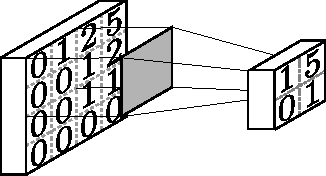
\includegraphics[width=.6\linewidth]{bg_pooling}
    \caption{Example of a Max Pooling Layer. For every 2 by 2 field the maximum is calculated. After applying first the convolution and then the pooling layer the information "T in the top right corner" is still there and size of the resulting matrix is very manageable.}
    \label{fig:bg:pooling}
\end{figure}

\paragraph{Example Network Architecture}
Now all the building blocks for a complete ConvNet are available. Repeatedly alternating convolution and pooling layers changes the input from wide in x and y dimension and narrow in z to a long z-strip. At the very end this strip is fed into one densely connected layer which is in turn connected to the output neurons. An example architecture of this kind is shown in figure \ref{fig:bg:NN_example}:

\begin{figure}[H]
    \centering
    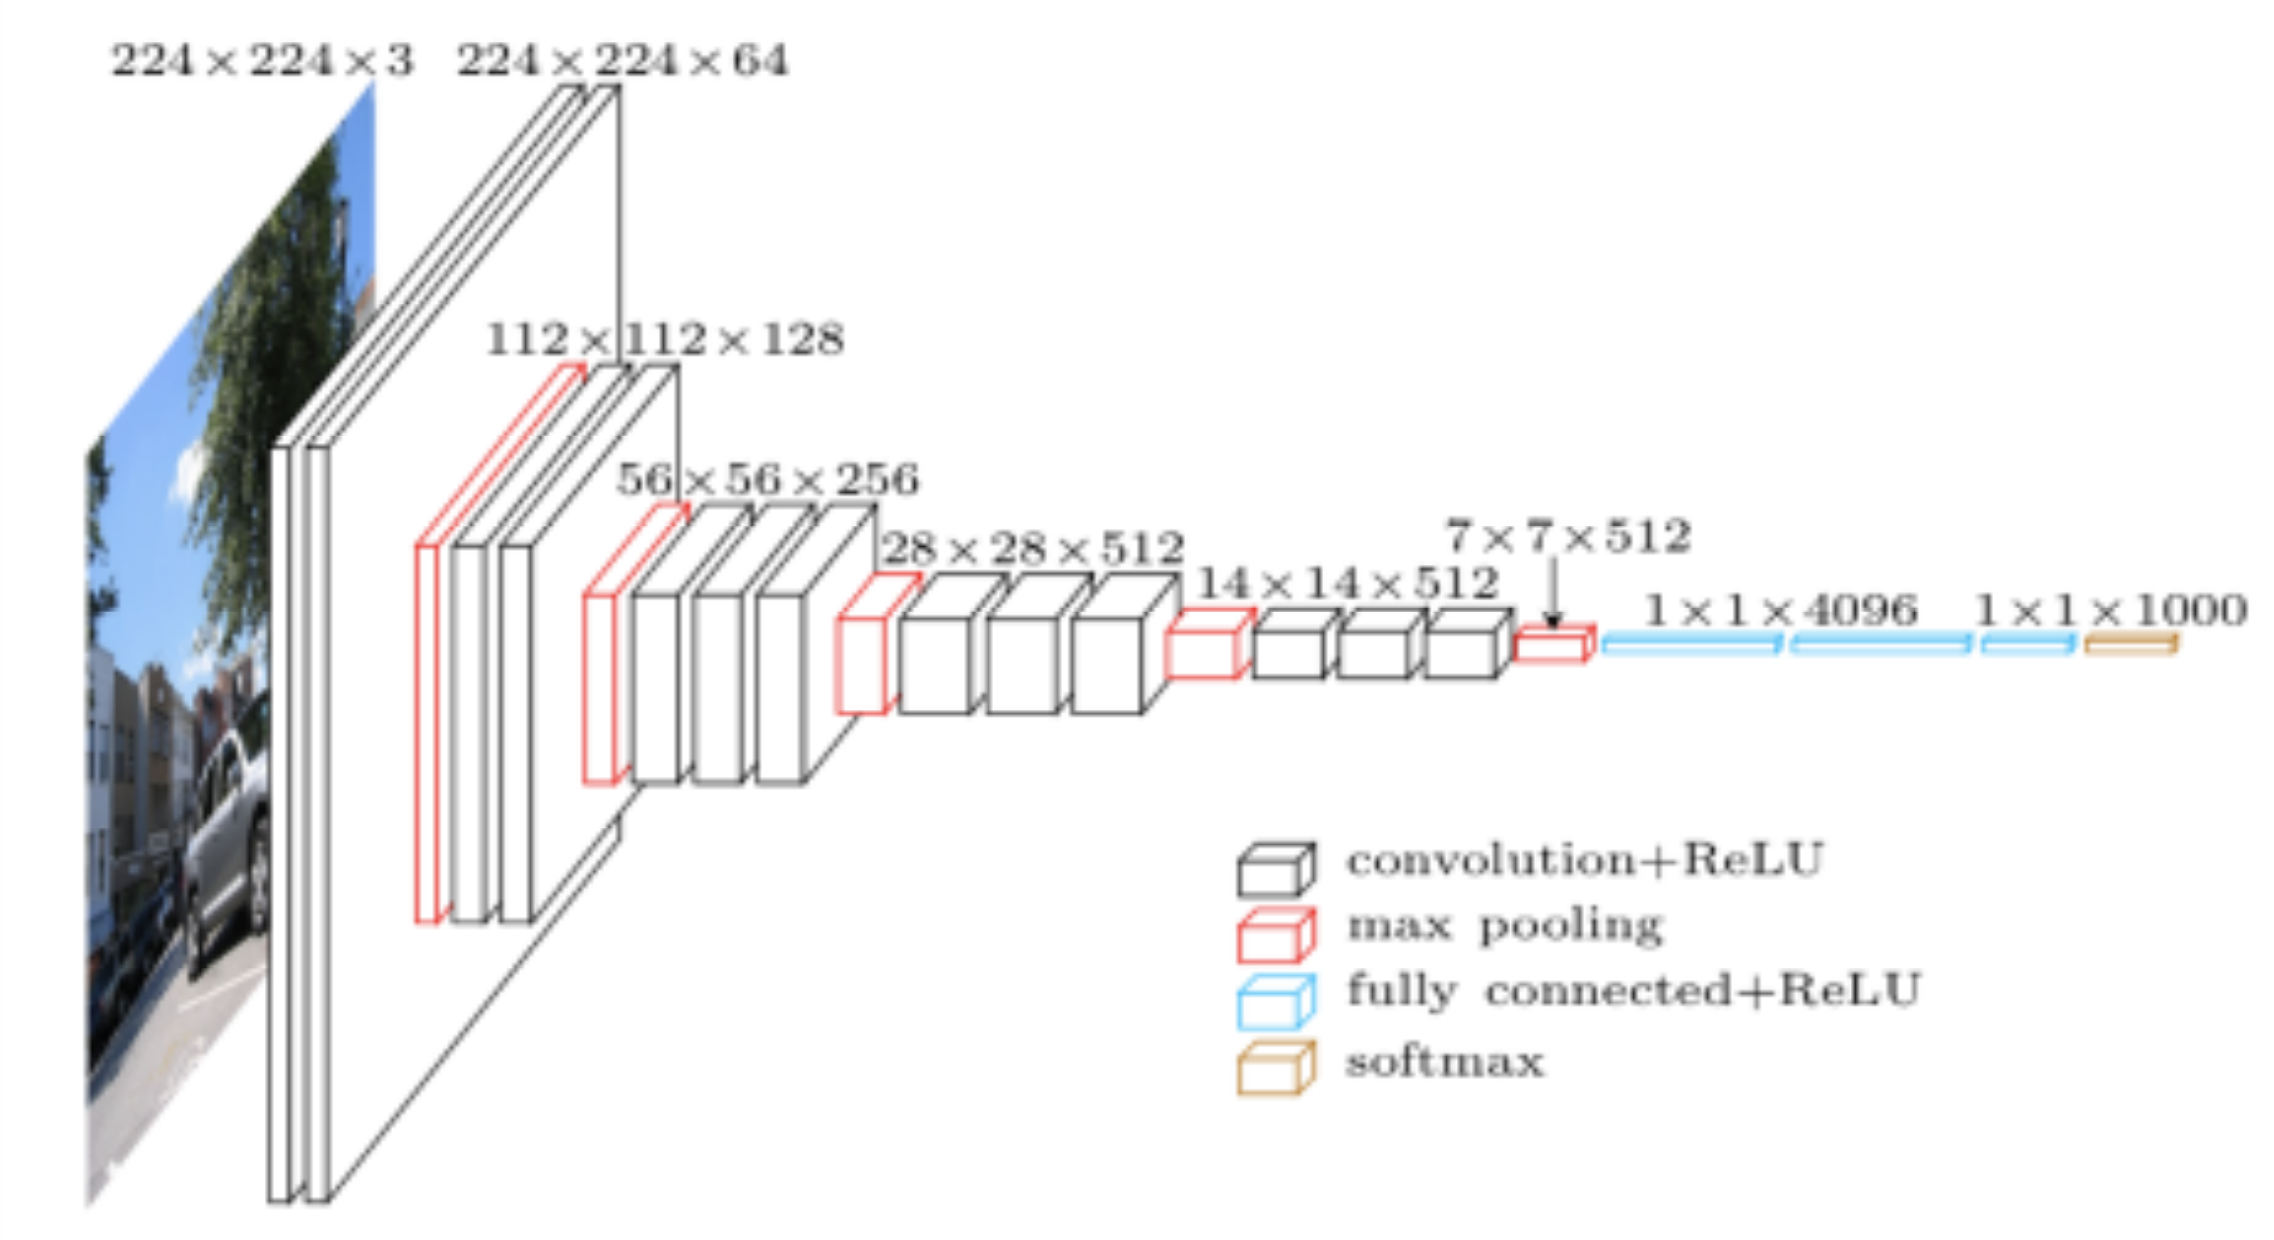
\includegraphics[width=.8\linewidth]{conv_net_example}
    \caption{Example for a complete ConvNet. Note the input is in this case an RGB image so there are three layers in the z dimension corresponding to the different colors. In this case the first layer has 64 kernels of size $3 \times 3 \times 3$. The next convolution then has 128 kernels of size $3 \times 3 \times 64$. [citation needed]}
    \label{fig:bg:NN_example}
\end{figure}


\paragraph{1D ConvNets}
The input to the desired algorithm is a target spectrum to which the Network should output some parameters (more on this in the section \ref{sec:NN}). This input data is a function $I(\lambda)$ so only one dimensional but all the same ideas apply. Convolutional kernels are sized $1 \times 3 \times z$ and pooling kernels are $1 \times 2 \times z$. Both are  only shifted in one direction as see in figure \ref{fig:bg:1D_conv}. These 1D convolutions might detect features like rising and falling edges and the later layers might combine these features into concepts like peaks and troughs but as always in machine learning what the network actually does to reach its objective is not controlled by the programmer.

\begin{figure}[H]
    \centering
    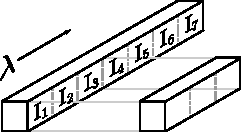
\includegraphics[width=.4\linewidth]{bg_1D_conv}
    \caption{Example of a 1D convolution. A $1 \times 3$ kernel is shifted over a spectrum $I$ discretized at 9 wavelengths}
    \label{fig:bg:1D_conv}
\end{figure}

\paragraph{Dropout Layer}
In 2014 Srivastava et al.\cite{Srivastava2014} presented a method to prevent overfitting and speed up the training process of large Neural Networks. During training they randomly drop a number of neurons in a layer along with all connections to and from these neurons. This prevents the neurons from co-adapting \note{explain co-adapting} and because there are less weights and biases to tune for each step the training becomes overall faster. The process of dropping some neurons is shown in figure \ref{fig:bg:dropout}:

\begin{figure}[H]
\centering
\begin{subfigure}{.5\textwidth}
    \centering
    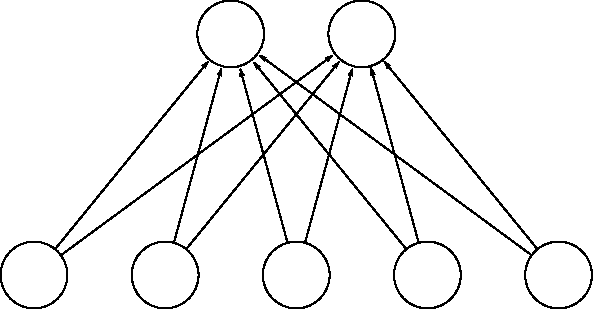
\includegraphics[width=.9\linewidth]{bg_no_dropout}
    \caption{no dropout}
    \label{}
\end{subfigure}%
\begin{subfigure}{.5\textwidth}
    \centering
    \includegraphics[width=.9\linewidth]{bg_dropout}
    \caption{with dropout}
    \label{}
\end{subfigure}
\caption{Example of a dropout applied to the bottom layer. Only two of the neurons remain active and only their weights and biases are modified during this training step. Figure found in \cite{Srivastava2014} (modified)}
\label{fig:bg:dropout}
\end{figure}
